% Author	Rajath Shashidhara
% Email		rajath.shashidhara@gmail.com
%
% This work is licensed under the Creative Commons Attribution 4.0 International License. 
% To view a copy of this license, visit http://creativecommons.org/licenses/by/4.0/.

\chapter{AAH model driven by Linearly Polarized Light}
We drive the AAH system by an electric field oriented along one of the lattice vector directions. The motivation for such a model is that it presents a more accurate description
of the Quantum Hall effect. Magnetic field in the plane of the lattice does not affect the motion of electrons restricted to 2-dimensional lattice (from Lorentz's force law). Therefore,
this feature of linearly polarized light may be effectively ignored.

Adding an electric field that is constant across the space does not change the periodicity properties of the Hamiltonian. The magnetic translation vectors are multiplied by a
constant phase factor and the magnetic translation group can be defined on the same lines as the pure AAH case. Correspondingly, the q-subband structure is not affected by this driving.

The magnetic vector potential corresponding to the system is
\begin{equation}
 \mathbf{A}(t) = (Bx + A\cos(\omega t)) \hat{\mathbf{y}}
\end{equation}
Using Peirels substitution as shown in Chapter \ref{ch:aah}, the Hamiltonian in the tight-binding form can be obtained.
\section{Effective Hamiltonian}
Following the same presciption detailed in Chapter \ref{ch:aah}, the Hamiltonian in real space is represented by the recursive equation
\begin{equation}
 a_{n+1} + a_{n-1} + 2\lambda\cos(2\pi(\alpha_0 + \alpha \cos{\omega t}) + \theta) a_{n} = E a_{n}
\end{equation} where $\alpha_0 = \frac{e}{h}Bd^2$ and $\alpha = \frac{e}{h}Ad$.

To proceed further, we shall apply the Floquet-BW perturbation theory to obtain the time-independent effective Hamiltonian.
Using the trignometric results listed in Appendix \ref{app:trig}, the fourier components of the Hamiltonian are
\begin{equation}
 H^{m,n}_{i,j} = \begin{cases}
            \delta_{i+1,j} + \delta_{i,j+1} + 2\lambda \mathcal{J}_{0}(2\pi\alpha) \cos(\theta + 2\pi\alpha_0 j) \;\delta_{i,j} & m=n\\
            (-1)^{\frac{|m-n|}{2}} \;2\lambda \mathcal{J}_{|m-n|}(2\pi\alpha) \cos(\theta + 2\pi\alpha_0 j) \;\delta_{i,j} & |m-n| \text{ is even}\\
            (-1)^{\frac{|m-n|+1}{2}} \;2\lambda \mathcal{J}_{|m-n|}(2\pi\alpha) \sin(\theta + 2\pi\alpha_0 j) \;\delta_{i,j} & |m-n| \text{ is odd}
           \end{cases}
\end{equation}
$H_{BW}^{(1)}$  is zero because
\begin{equation*}
 \frac{H_{0,n}H_{n,0}}{n\omega} + \frac{H_{0,-n}H_{-n,0}}{(-n)\omega} = 0
\end{equation*}
$H_{BW}^{(2)}$ only contributes to diagonal terms because of the structure of fourier components detailed above.

The momentum space Hamiltonian for this problem can be derived using the same approach used in the pure AAH case.
\begin{equation}
 H(k_x, k_y, t)_{i,j} = \delta_{i+1,j} + \delta_{i,j+1} + 2\lambda\cos(k_y + 2\pi\alpha_0 j - 2\pi\alpha \cos{\omega t}) \delta_{i,j} + e^{-iqk_x} \delta_{i,1}\delta_{j,q} + e^{iqk_x} \delta_{i,q}\delta_{j,1}
\end{equation} where $k_x \in [-\pi/q, \pi/q]$, $k_y \in [-\pi,\pi]$ and $i,j \in 1\dots q$.
Consequently, the fourier components are
\begin{equation}
 H^{m,n}_{i,j}(k_x, k_y) = \begin{cases}
            \begin{split}\delta_{i+1,j} + \delta_{i,j+1} + e^{-iqk_x} \delta_{i,1}\delta_{j,q} + e^{iqk_x} \delta_{i,q}\delta_{j,1} \\+ 2\lambda \mathcal{J}_{0}(2\pi\alpha) \cos(\theta + 2\pi\alpha_0 j) \;\delta_{i,j}\end{split} & m=n\\
            (-1)^{\frac{|m-n|}{2}} \;2\lambda \mathcal{J}_{|m-n|}(2\pi\alpha) \cos(\theta + 2\pi\alpha_0 j) \;\delta_{i,j} & |m-n| \text{ is even}\\
            (-1)^{\frac{|m-n|-1}{2}} \;2\lambda \mathcal{J}_{|m-n|}(2\pi\alpha) \sin(\theta + 2\pi\alpha_0 j) \;\delta_{i,j} & |m-n| \text{ is odd}
           \end{cases}
\end{equation}
$H_{BW}$ is numerically computed from the above fourier components up to order $\mathcal{O}(1/\omega^3)$.
\section{Results}
We shall analyze the perturbation terms arising due to the linear electric field. The perturbation terms contribute to each lattice site uniformly i.e., they are independent of
the lattice site index. Further, they only affect the on-site terms. On-site terms are akin to potential energy assigned to each lattice site and off-site terms are hopping terms,
and they are indicators of kinetic energy due to hopping of electrons between neighbors in the lattice.

\begin{figure}[t]
 \centering
 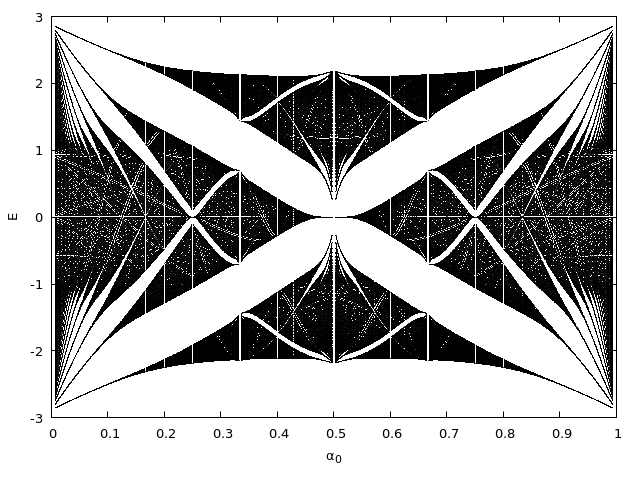
\includegraphics[width=0.65\textwidth]{linear-spectrum}\\
 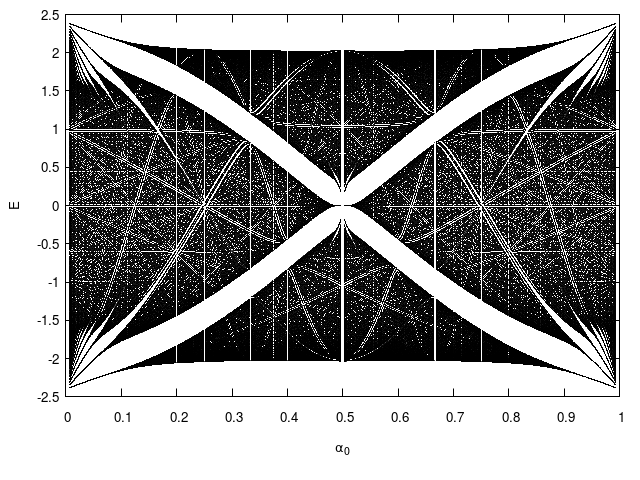
\includegraphics[width=0.65\textwidth]{linear-spectrum5}\\
 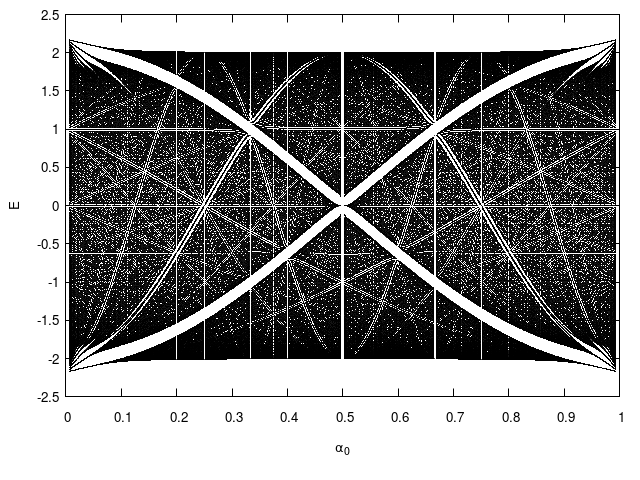
\includegraphics[width=0.65\textwidth]{linear-spectrum25}
 \caption{Spectrum of the driven Aubry-Andr\'e-Harper model by linearly polarized electric field. The parameters are set to $\lambda=1.0$, $\omega=1.0$ and $k_x=0, k_y=0$.
 (a) $\alpha = 1.0$ (b) $\alpha = 5.0$ (c) $\alpha = 25.0$}
\end{figure}

As the magnitude of electric field increases, the range of energy eigenvalues is diminishing and the gaps in the spectrum are compacted. The same effect can be achieved by increasing
the $\lambda$ in the pure AAH model. However, the perturbation terms include products of $\cos(\theta + 2\pi\alpha_0 j)$ and $\sin(\theta + 2\pi\alpha_0 j)$ accompanied by
oscillatory multiplicative factors in the form of bessel functions, to the on-site terms. It is nearly impossible to gauge the impact of the perturbation terms on
the recursive structure of the graph. Analysis of this nature requires mathematical skills beyond the abilities of the author at the time of writing this document.

We examine the nature of metal-insulator transition for ground state of real-space Hamiltonian using the plot of $IPR$ vs. $\lambda$ and $IPR$ vs. $\alpha$.
\begin{figure}[h]
 \centering
 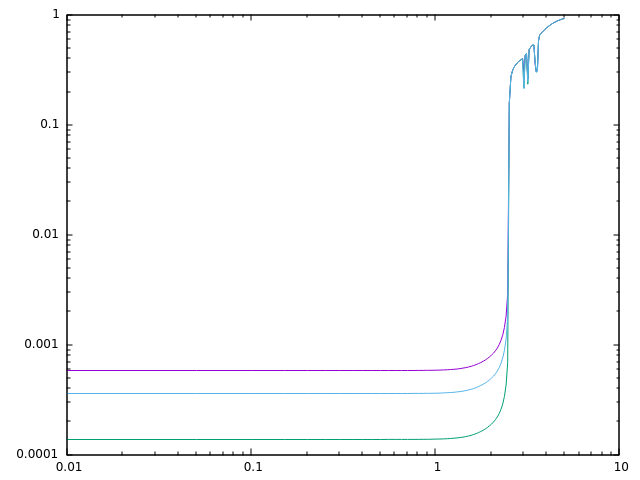
\includegraphics[width=0.45\textwidth]{ipr-linear}
 \caption{Plot of $IPR$ vs $\lambda$ for $L=2584,4181,10946$ and  $\alpha=1.0, \alpha_0=1/goldenratio$.}
\end{figure}

When the chern numbers are plotted against $\alpha$, the topological transitions are unveiled. This discovery is quite intriguing as the transitions are periodic and they seem to
be independent of $\alpha_0$. Also, the width of transition is increasing as $\alpha$ increases. A deeper analysis of undergoing phenomenon must be carried out to understand the 
observations. This reported is limited to calculation of chern numbers. Analysis will be published in a future work.

The relationship between Chern numbers and Hall conductivity for time-dependent systems is non-trivial and requires further literature survey to understand it. This has not been 
taken up as a part of this thesis. However, a transition in chern number clearly indicates a topological transition and this in some way impacts the physical quantities.
\begin{figure}[h]
 \centering
 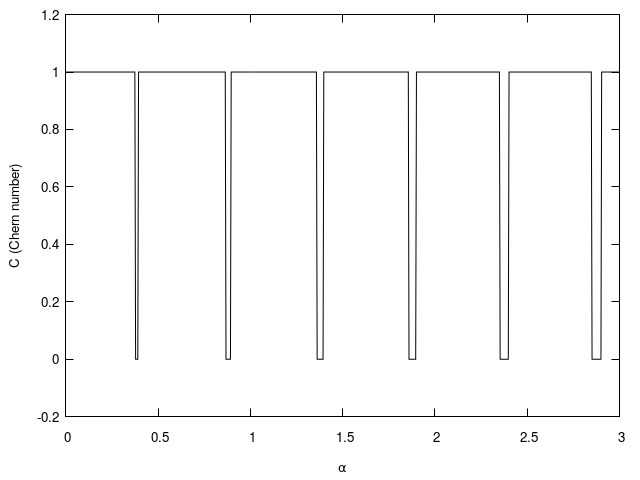
\includegraphics[width=0.45\textwidth]{linear-chern-3a}\\
 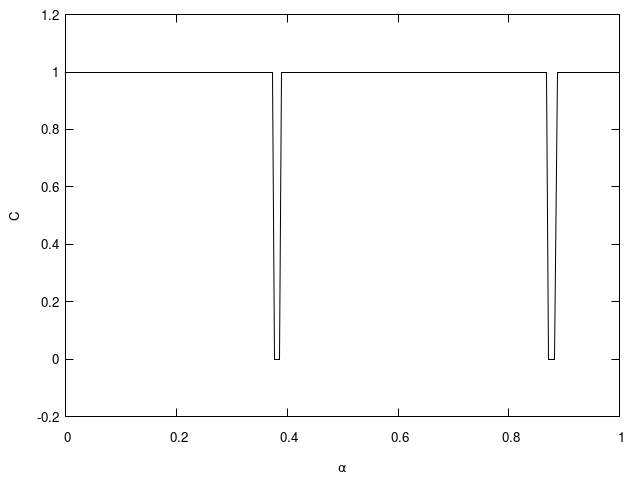
\includegraphics[width=0.45\textwidth]{linear-chern-5a}
 \caption{Plot of Chern numbers of the lowest subband vs. $\alpha$ for (a) $\alpha_0 = 1/3$ (b) $\alpha_0 = 1/5$.}
\end{figure}
